% Options for packages loaded elsewhere
\PassOptionsToPackage{unicode}{hyperref}
\PassOptionsToPackage{hyphens}{url}
\PassOptionsToPackage{dvipsnames,svgnames,x11names}{xcolor}
%
\documentclass[
  letterpaper,
  DIV=11,
  numbers=noendperiod]{scrartcl}

\usepackage{amsmath,amssymb}
\usepackage{iftex}
\ifPDFTeX
  \usepackage[T1]{fontenc}
  \usepackage[utf8]{inputenc}
  \usepackage{textcomp} % provide euro and other symbols
\else % if luatex or xetex
  \usepackage{unicode-math}
  \defaultfontfeatures{Scale=MatchLowercase}
  \defaultfontfeatures[\rmfamily]{Ligatures=TeX,Scale=1}
\fi
\usepackage{lmodern}
\ifPDFTeX\else  
    % xetex/luatex font selection
\fi
% Use upquote if available, for straight quotes in verbatim environments
\IfFileExists{upquote.sty}{\usepackage{upquote}}{}
\IfFileExists{microtype.sty}{% use microtype if available
  \usepackage[]{microtype}
  \UseMicrotypeSet[protrusion]{basicmath} % disable protrusion for tt fonts
}{}
\makeatletter
\@ifundefined{KOMAClassName}{% if non-KOMA class
  \IfFileExists{parskip.sty}{%
    \usepackage{parskip}
  }{% else
    \setlength{\parindent}{0pt}
    \setlength{\parskip}{6pt plus 2pt minus 1pt}}
}{% if KOMA class
  \KOMAoptions{parskip=half}}
\makeatother
\usepackage{xcolor}
\setlength{\emergencystretch}{3em} % prevent overfull lines
\setcounter{secnumdepth}{5}
% Make \paragraph and \subparagraph free-standing
\makeatletter
\ifx\paragraph\undefined\else
  \let\oldparagraph\paragraph
  \renewcommand{\paragraph}{
    \@ifstar
      \xxxParagraphStar
      \xxxParagraphNoStar
  }
  \newcommand{\xxxParagraphStar}[1]{\oldparagraph*{#1}\mbox{}}
  \newcommand{\xxxParagraphNoStar}[1]{\oldparagraph{#1}\mbox{}}
\fi
\ifx\subparagraph\undefined\else
  \let\oldsubparagraph\subparagraph
  \renewcommand{\subparagraph}{
    \@ifstar
      \xxxSubParagraphStar
      \xxxSubParagraphNoStar
  }
  \newcommand{\xxxSubParagraphStar}[1]{\oldsubparagraph*{#1}\mbox{}}
  \newcommand{\xxxSubParagraphNoStar}[1]{\oldsubparagraph{#1}\mbox{}}
\fi
\makeatother

\usepackage{color}
\usepackage{fancyvrb}
\newcommand{\VerbBar}{|}
\newcommand{\VERB}{\Verb[commandchars=\\\{\}]}
\DefineVerbatimEnvironment{Highlighting}{Verbatim}{commandchars=\\\{\}}
% Add ',fontsize=\small' for more characters per line
\usepackage{framed}
\definecolor{shadecolor}{RGB}{241,243,245}
\newenvironment{Shaded}{\begin{snugshade}}{\end{snugshade}}
\newcommand{\AlertTok}[1]{\textcolor[rgb]{0.68,0.00,0.00}{#1}}
\newcommand{\AnnotationTok}[1]{\textcolor[rgb]{0.37,0.37,0.37}{#1}}
\newcommand{\AttributeTok}[1]{\textcolor[rgb]{0.40,0.45,0.13}{#1}}
\newcommand{\BaseNTok}[1]{\textcolor[rgb]{0.68,0.00,0.00}{#1}}
\newcommand{\BuiltInTok}[1]{\textcolor[rgb]{0.00,0.23,0.31}{#1}}
\newcommand{\CharTok}[1]{\textcolor[rgb]{0.13,0.47,0.30}{#1}}
\newcommand{\CommentTok}[1]{\textcolor[rgb]{0.37,0.37,0.37}{#1}}
\newcommand{\CommentVarTok}[1]{\textcolor[rgb]{0.37,0.37,0.37}{\textit{#1}}}
\newcommand{\ConstantTok}[1]{\textcolor[rgb]{0.56,0.35,0.01}{#1}}
\newcommand{\ControlFlowTok}[1]{\textcolor[rgb]{0.00,0.23,0.31}{\textbf{#1}}}
\newcommand{\DataTypeTok}[1]{\textcolor[rgb]{0.68,0.00,0.00}{#1}}
\newcommand{\DecValTok}[1]{\textcolor[rgb]{0.68,0.00,0.00}{#1}}
\newcommand{\DocumentationTok}[1]{\textcolor[rgb]{0.37,0.37,0.37}{\textit{#1}}}
\newcommand{\ErrorTok}[1]{\textcolor[rgb]{0.68,0.00,0.00}{#1}}
\newcommand{\ExtensionTok}[1]{\textcolor[rgb]{0.00,0.23,0.31}{#1}}
\newcommand{\FloatTok}[1]{\textcolor[rgb]{0.68,0.00,0.00}{#1}}
\newcommand{\FunctionTok}[1]{\textcolor[rgb]{0.28,0.35,0.67}{#1}}
\newcommand{\ImportTok}[1]{\textcolor[rgb]{0.00,0.46,0.62}{#1}}
\newcommand{\InformationTok}[1]{\textcolor[rgb]{0.37,0.37,0.37}{#1}}
\newcommand{\KeywordTok}[1]{\textcolor[rgb]{0.00,0.23,0.31}{\textbf{#1}}}
\newcommand{\NormalTok}[1]{\textcolor[rgb]{0.00,0.23,0.31}{#1}}
\newcommand{\OperatorTok}[1]{\textcolor[rgb]{0.37,0.37,0.37}{#1}}
\newcommand{\OtherTok}[1]{\textcolor[rgb]{0.00,0.23,0.31}{#1}}
\newcommand{\PreprocessorTok}[1]{\textcolor[rgb]{0.68,0.00,0.00}{#1}}
\newcommand{\RegionMarkerTok}[1]{\textcolor[rgb]{0.00,0.23,0.31}{#1}}
\newcommand{\SpecialCharTok}[1]{\textcolor[rgb]{0.37,0.37,0.37}{#1}}
\newcommand{\SpecialStringTok}[1]{\textcolor[rgb]{0.13,0.47,0.30}{#1}}
\newcommand{\StringTok}[1]{\textcolor[rgb]{0.13,0.47,0.30}{#1}}
\newcommand{\VariableTok}[1]{\textcolor[rgb]{0.07,0.07,0.07}{#1}}
\newcommand{\VerbatimStringTok}[1]{\textcolor[rgb]{0.13,0.47,0.30}{#1}}
\newcommand{\WarningTok}[1]{\textcolor[rgb]{0.37,0.37,0.37}{\textit{#1}}}

\providecommand{\tightlist}{%
  \setlength{\itemsep}{0pt}\setlength{\parskip}{0pt}}\usepackage{longtable,booktabs,array}
\usepackage{calc} % for calculating minipage widths
% Correct order of tables after \paragraph or \subparagraph
\usepackage{etoolbox}
\makeatletter
\patchcmd\longtable{\par}{\if@noskipsec\mbox{}\fi\par}{}{}
\makeatother
% Allow footnotes in longtable head/foot
\IfFileExists{footnotehyper.sty}{\usepackage{footnotehyper}}{\usepackage{footnote}}
\makesavenoteenv{longtable}
\usepackage{graphicx}
\makeatletter
\newsavebox\pandoc@box
\newcommand*\pandocbounded[1]{% scales image to fit in text height/width
  \sbox\pandoc@box{#1}%
  \Gscale@div\@tempa{\textheight}{\dimexpr\ht\pandoc@box+\dp\pandoc@box\relax}%
  \Gscale@div\@tempb{\linewidth}{\wd\pandoc@box}%
  \ifdim\@tempb\p@<\@tempa\p@\let\@tempa\@tempb\fi% select the smaller of both
  \ifdim\@tempa\p@<\p@\scalebox{\@tempa}{\usebox\pandoc@box}%
  \else\usebox{\pandoc@box}%
  \fi%
}
% Set default figure placement to htbp
\def\fps@figure{htbp}
\makeatother

\KOMAoption{captions}{tableheading}
\makeatletter
\@ifpackageloaded{caption}{}{\usepackage{caption}}
\AtBeginDocument{%
\ifdefined\contentsname
  \renewcommand*\contentsname{Table of contents}
\else
  \newcommand\contentsname{Table of contents}
\fi
\ifdefined\listfigurename
  \renewcommand*\listfigurename{List of Figures}
\else
  \newcommand\listfigurename{List of Figures}
\fi
\ifdefined\listtablename
  \renewcommand*\listtablename{List of Tables}
\else
  \newcommand\listtablename{List of Tables}
\fi
\ifdefined\figurename
  \renewcommand*\figurename{Figure}
\else
  \newcommand\figurename{Figure}
\fi
\ifdefined\tablename
  \renewcommand*\tablename{Table}
\else
  \newcommand\tablename{Table}
\fi
}
\@ifpackageloaded{float}{}{\usepackage{float}}
\floatstyle{ruled}
\@ifundefined{c@chapter}{\newfloat{codelisting}{h}{lop}}{\newfloat{codelisting}{h}{lop}[chapter]}
\floatname{codelisting}{Listing}
\newcommand*\listoflistings{\listof{codelisting}{List of Listings}}
\makeatother
\makeatletter
\makeatother
\makeatletter
\@ifpackageloaded{caption}{}{\usepackage{caption}}
\@ifpackageloaded{subcaption}{}{\usepackage{subcaption}}
\makeatother

\usepackage{bookmark}

\IfFileExists{xurl.sty}{\usepackage{xurl}}{} % add URL line breaks if available
\urlstyle{same} % disable monospaced font for URLs
\hypersetup{
  pdftitle={4. Übungsblatt (Faktorielle Umfrageexperimente)},
  pdfauthor={Daria Tisch},
  colorlinks=true,
  linkcolor={blue},
  filecolor={Maroon},
  citecolor={Blue},
  urlcolor={Blue},
  pdfcreator={LaTeX via pandoc}}


\title{4. Übungsblatt (Faktorielle Umfrageexperimente)}
\author{Daria Tisch}
\date{}

\begin{document}
\maketitle


\section{Organisation}\label{organisation}

\subsection{Arbeitsverzeichnis
festsetzen}\label{arbeitsverzeichnis-festsetzen}

\subsection{Packages installieren und
laden}\label{packages-installieren-und-laden}

\begin{Shaded}
\begin{Highlighting}[]
\CommentTok{\# Packages}
\NormalTok{pkgs }\OtherTok{\textless{}{-}} \FunctionTok{c}\NormalTok{(}
  \StringTok{"tidyverse"}\NormalTok{,}
  \StringTok{"sjPlot"}\NormalTok{,}
  \StringTok{"haven"}\NormalTok{,}
  \StringTok{"labelled"}\NormalTok{ ,}
  \StringTok{"sandwich"}\NormalTok{,}
  \StringTok{"lmtest"}\NormalTok{,}
  \StringTok{"Hmisc"}
\NormalTok{) }

\DocumentationTok{\#\# Install uninstalled packages}
\FunctionTok{lapply}\NormalTok{(pkgs[}\SpecialCharTok{!}\NormalTok{(pkgs }\SpecialCharTok{\%in\%} \FunctionTok{installed.packages}\NormalTok{())], install.packages)}

\DocumentationTok{\#\# Load all packages to library}
\FunctionTok{lapply}\NormalTok{(pkgs, library, }\AttributeTok{character.only =} \ConstantTok{TRUE}\NormalTok{)}
\end{Highlighting}
\end{Shaded}

\subsection{Einführung}\label{einfuxfchrung}

In dieser Übung replizieren wir die Ergebnisse folgender Studie:

Tisch, Daria, and Tamara Gutfleisch. `Unequal but Just? Experimental
Evidence on Distributive Justice Principles in Parental Inter Vivos
Transfers'. Socio-Economic Review 21, no. 3 (2023): 1369--90.

Der Datensatz kann
\href{https://dariatisch.github.io/wup2024/downloads/just_transfers.csv}{hier}
heruntergeladen werden.

Schenkungen von Eltern an deren Kinder sind von der moralischen
Entscheidung geprägt, welches Kind wie viel erhalten soll. So können
Eltern Schenkungen zwischen Kindern nach unterschiedlichen
Gerechtigkeitsprinzipien aufteilen. Wenden sie das Gleichheitsprinzip
an, schenken sie allen Kindern gleich viel. Wenden sie das
Bedürfnisprinzip an, schenken sie den Kindern, die größere Bedürfnisse
haben (z. B. Arbeitslosigkeit), mehr. Wenden sie das Austauschprinzip
an, schenken sie den Kindern mehr, die im Gegenzug mehr für die Eltern
machen (z. B. im Haushalt der Eltern helfen). Wenden sie das
Anspruchsprinzip an, schenken sie den Kindern mehr, die bestimmte
angeborene Statuscharakteristiken haben (z. B. Erstgeborene). Wir wollen
untersuchen, inwiefern diese Prinzipien im Kontext von elterlichen
Schenkungen von den Befragten befürwortet werden. Unterstützen die
Befragten diese Prinzipien im selben Maße für Töchter und Söhne?

\subsection{Daten einlesen}\label{daten-einlesen}

\begin{Shaded}
\begin{Highlighting}[]
\CommentTok{\# Load the data file}
\NormalTok{df }\OtherTok{\textless{}{-}} \FunctionTok{read.csv}\NormalTok{(}\StringTok{"daten/just\_transfers.csv"}\NormalTok{)}
\end{Highlighting}
\end{Shaded}

\subsection{Variablenlabels einlesen}\label{variablenlabels-einlesen}

\begin{Shaded}
\begin{Highlighting}[]
\CommentTok{\# Load the variable labels}
\NormalTok{variable\_labels }\OtherTok{\textless{}{-}} \FunctionTok{read.csv}\NormalTok{(}\StringTok{"daten/just\_transfers\_variable\_labels.csv"}\NormalTok{, }\AttributeTok{row.names =} \DecValTok{1}\NormalTok{, }\AttributeTok{stringsAsFactors =} \ConstantTok{FALSE}\NormalTok{)}

\CommentTok{\# View variable labels}
\CommentTok{\#print(variable\_labels)}


\CommentTok{\# Loop through the labels and assign them to variables in the dataset}
\ControlFlowTok{for}\NormalTok{ (var }\ControlFlowTok{in} \FunctionTok{names}\NormalTok{(variable\_labels)) \{}
  \ControlFlowTok{if}\NormalTok{ (var }\SpecialCharTok{\%in\%} \FunctionTok{names}\NormalTok{(df)) \{}
    \FunctionTok{var\_label}\NormalTok{(df[[var]]) }\OtherTok{\textless{}{-}}\NormalTok{ variable\_labels[[var]]}
\NormalTok{  \}}
\NormalTok{\}}
\end{Highlighting}
\end{Shaded}

\subsection{Value labels einlesen}\label{value-labels-einlesen}

\begin{Shaded}
\begin{Highlighting}[]
\CommentTok{\# Load the value labels}
\NormalTok{value\_labels }\OtherTok{\textless{}{-}} \FunctionTok{read.csv}\NormalTok{(}\StringTok{"daten/value\_labels.csv"}\NormalTok{, }\AttributeTok{stringsAsFactors =} \ConstantTok{FALSE}\NormalTok{)}

\CommentTok{\# View value labels}
\FunctionTok{head}\NormalTok{(value\_labels)}
\end{Highlighting}
\end{Shaded}

\begin{verbatim}
   variable               label value
1 firstborn       Son firstborn     1
2 firstborn               Twins     2
3 firstborn  Daughter firstborn     3
4      need      Son unemployed     1
5      need      Equal earnings     2
6      need Daughter unemployed     3
\end{verbatim}

\section{Kennenlernen des
Datensatzes}\label{kennenlernen-des-datensatzes}

\subsection{Wie viele Beobachtungen enthält der
Datensatz?}\label{wie-viele-beobachtungen-enthuxe4lt-der-datensatz}

\begin{Shaded}
\begin{Highlighting}[]
\FunctionTok{nrow}\NormalTok{(df)}
\end{Highlighting}
\end{Shaded}

\begin{verbatim}
[1] 4284
\end{verbatim}

\subsection{Wie viele befragte Personen sind im Datensatz
enthalten?}\label{wie-viele-befragte-personen-sind-im-datensatz-enthalten}

\begin{Shaded}
\begin{Highlighting}[]
\FunctionTok{length}\NormalTok{(}\FunctionTok{unique}\NormalTok{(df}\SpecialCharTok{$}\NormalTok{id\_resp))}
\end{Highlighting}
\end{Shaded}

\begin{verbatim}
[1] 714
\end{verbatim}

\subsection{Wie viele Vignetten hat jede befragte Person
bewertet?}\label{wie-viele-vignetten-hat-jede-befragte-person-bewertet}

\begin{Shaded}
\begin{Highlighting}[]
\FunctionTok{length}\NormalTok{(}\FunctionTok{unique}\NormalTok{(df}\SpecialCharTok{$}\NormalTok{id\_within))}
\end{Highlighting}
\end{Shaded}

\begin{verbatim}
[1] 3
\end{verbatim}

\begin{Shaded}
\begin{Highlighting}[]
\FunctionTok{table}\NormalTok{(df}\SpecialCharTok{$}\NormalTok{id\_within)}
\end{Highlighting}
\end{Shaded}

\begin{verbatim}

   1    2    3 
1428 1428 1428 
\end{verbatim}

\begin{Shaded}
\begin{Highlighting}[]
\DecValTok{1428}\SpecialCharTok{/}\DecValTok{2}
\end{Highlighting}
\end{Shaded}

\begin{verbatim}
[1] 714
\end{verbatim}

\subsection{Wie viele Vignetten gibt
es?}\label{wie-viele-vignetten-gibt-es}

\begin{Shaded}
\begin{Highlighting}[]
\FunctionTok{table}\NormalTok{(df}\SpecialCharTok{$}\NormalTok{id\_vignette)}
\end{Highlighting}
\end{Shaded}

\begin{verbatim}

  1   2   3   4   5   6   7   8   9  10  11  12  13  14  15  16  17  18  19  20 
134 134 134 162 162 162 180 180 180 168 168 168 146 146 146 174 174 174 154 154 
 21  22  23  24  25  26  27 
154 152 152 152 158 158 158 
\end{verbatim}

\begin{Shaded}
\begin{Highlighting}[]
\FunctionTok{length}\NormalTok{(}\FunctionTok{unique}\NormalTok{(df}\SpecialCharTok{$}\NormalTok{id\_vignette))}
\end{Highlighting}
\end{Shaded}

\begin{verbatim}
[1] 27
\end{verbatim}

\subsection{Wie viele Decks gibt es?}\label{wie-viele-decks-gibt-es}

\begin{Shaded}
\begin{Highlighting}[]
\FunctionTok{table}\NormalTok{(df}\SpecialCharTok{$}\NormalTok{deck)}
\end{Highlighting}
\end{Shaded}

\begin{verbatim}

  1   2   3   4   5   6   7   8   9 
402 486 540 504 438 522 462 456 474 
\end{verbatim}

\begin{Shaded}
\begin{Highlighting}[]
\FunctionTok{length}\NormalTok{(}\FunctionTok{unique}\NormalTok{(df}\SpecialCharTok{$}\NormalTok{deck))}
\end{Highlighting}
\end{Shaded}

\begin{verbatim}
[1] 9
\end{verbatim}

\subsection{Dimensionen und
Ausprägungen}\label{dimensionen-und-auspruxe4gungen}

Welche Dimensionen gibt es und welche Ausprägungen können diese
aufweisen? Tipp: Nutze den Datensatz: value\_labels

\begin{Shaded}
\begin{Highlighting}[]
\FunctionTok{head}\NormalTok{(value\_labels, }\DecValTok{9}\NormalTok{)}
\end{Highlighting}
\end{Shaded}

\begin{verbatim}
   variable               label value
1 firstborn       Son firstborn     1
2 firstborn               Twins     2
3 firstborn  Daughter firstborn     3
4      need      Son unemployed     1
5      need      Equal earnings     2
6      need Daughter unemployed     3
7      help           Son helps     1
8      help           Both help     2
9      help      Daughter helps     3
\end{verbatim}

\section{Orthogonalität und
Balance}\label{orthogonalituxe4t-und-balance}

\subsection{Sind die Dimensionen
orthogonal?}\label{sind-die-dimensionen-orthogonal}

\begin{Shaded}
\begin{Highlighting}[]
\CommentTok{\# Dummy{-}Variablen mit dplyr erstellen}
\NormalTok{df }\OtherTok{\textless{}{-}}\NormalTok{ df }\SpecialCharTok{\%\textgreater{}\%}
  \FunctionTok{mutate}\NormalTok{(}
    \CommentTok{\# Dummy{-}Variablen für firstborn}
    \AttributeTok{firstborn\_1 =} \FunctionTok{if\_else}\NormalTok{(firstborn }\SpecialCharTok{==} \DecValTok{1}\NormalTok{, }\DecValTok{1}\NormalTok{, }\DecValTok{0}\NormalTok{),}
    \AttributeTok{firstborn\_2 =} \FunctionTok{if\_else}\NormalTok{(firstborn }\SpecialCharTok{==} \DecValTok{2}\NormalTok{, }\DecValTok{1}\NormalTok{, }\DecValTok{0}\NormalTok{),}
    \AttributeTok{firstborn\_3 =} \FunctionTok{if\_else}\NormalTok{(firstborn }\SpecialCharTok{==} \DecValTok{3}\NormalTok{, }\DecValTok{1}\NormalTok{, }\DecValTok{0}\NormalTok{),}
    
    \CommentTok{\# Dummy{-}Variablen für help}
    \AttributeTok{help\_1 =} \FunctionTok{if\_else}\NormalTok{(help }\SpecialCharTok{==} \DecValTok{1}\NormalTok{, }\DecValTok{1}\NormalTok{, }\DecValTok{0}\NormalTok{),}
    \AttributeTok{help\_2 =} \FunctionTok{if\_else}\NormalTok{(help }\SpecialCharTok{==} \DecValTok{2}\NormalTok{, }\DecValTok{1}\NormalTok{, }\DecValTok{0}\NormalTok{),}
    \AttributeTok{help\_3 =} \FunctionTok{if\_else}\NormalTok{(help }\SpecialCharTok{==} \DecValTok{3}\NormalTok{, }\DecValTok{1}\NormalTok{, }\DecValTok{0}\NormalTok{),}
    
    \CommentTok{\# Dummy{-}Variablen für need}
    \AttributeTok{need\_1 =} \FunctionTok{if\_else}\NormalTok{(need }\SpecialCharTok{==} \DecValTok{1}\NormalTok{, }\DecValTok{1}\NormalTok{, }\DecValTok{0}\NormalTok{),}
    \AttributeTok{need\_2 =} \FunctionTok{if\_else}\NormalTok{(need }\SpecialCharTok{==} \DecValTok{2}\NormalTok{, }\DecValTok{1}\NormalTok{, }\DecValTok{0}\NormalTok{),}
    \AttributeTok{need\_3 =} \FunctionTok{if\_else}\NormalTok{(need }\SpecialCharTok{==} \DecValTok{3}\NormalTok{, }\DecValTok{1}\NormalTok{, }\DecValTok{0}\NormalTok{)}
\NormalTok{  )}


\CommentTok{\# Select relevant columns}
\NormalTok{selected\_columns }\OtherTok{\textless{}{-}}\NormalTok{ df[, }\FunctionTok{c}\NormalTok{(}\StringTok{"firstborn\_1"}\NormalTok{, }
                           \StringTok{"firstborn\_2"}\NormalTok{,}
                           \StringTok{"firstborn\_3"}\NormalTok{,}
                           \StringTok{"need\_1"}\NormalTok{,}
                           \StringTok{"need\_2"}\NormalTok{,}
                           \StringTok{"need\_3"}\NormalTok{,}
                           \StringTok{"help\_1"}\NormalTok{,}
                           \StringTok{"help\_2"}\NormalTok{, }
                           \StringTok{"help\_3"}\NormalTok{)]}

\CommentTok{\# Compute pairwise correlations with significance}
\NormalTok{cor\_results }\OtherTok{\textless{}{-}} \FunctionTok{rcorr}\NormalTok{(}\FunctionTok{as.matrix}\NormalTok{(selected\_columns))}

\CommentTok{\# Display results}
\FunctionTok{print}\NormalTok{(cor\_results)}
\end{Highlighting}
\end{Shaded}

\begin{verbatim}
            firstborn_1 firstborn_2 firstborn_3 need_1 need_2 need_3 help_1
firstborn_1        1.00       -0.50       -0.50   0.02  -0.01  -0.01   0.04
firstborn_2       -0.50        1.00       -0.50   0.01  -0.02   0.00  -0.01
firstborn_3       -0.50       -0.50        1.00  -0.03   0.03   0.01  -0.03
need_1             0.02        0.01       -0.03   1.00  -0.50  -0.50  -0.01
need_2            -0.01       -0.02        0.03  -0.50   1.00  -0.50  -0.01
need_3            -0.01        0.00        0.01  -0.50  -0.50   1.00   0.02
help_1             0.04       -0.01       -0.03  -0.01  -0.01   0.02   1.00
help_2             0.00       -0.02        0.02   0.02  -0.01  -0.01  -0.50
help_3            -0.04        0.04        0.01  -0.01   0.02  -0.01  -0.50
            help_2 help_3
firstborn_1   0.00  -0.04
firstborn_2  -0.02   0.04
firstborn_3   0.02   0.01
need_1        0.02  -0.01
need_2       -0.01   0.02
need_3       -0.01  -0.01
help_1       -0.50  -0.50
help_2        1.00  -0.50
help_3       -0.50   1.00

n= 4284 


P
            firstborn_1 firstborn_2 firstborn_3 need_1 need_2 need_3 help_1
firstborn_1             0.0000      0.0000      0.2160 0.5824 0.4919 0.0060
firstborn_2 0.0000                  0.0000      0.4095 0.2714 0.7834 0.4095
firstborn_3 0.0000      0.0000                  0.0392 0.0990 0.6800 0.0542
need_1      0.2160      0.4095      0.0392             0.0000 0.0000 0.4919
need_2      0.5824      0.2714      0.0990      0.0000        0.0000 0.4919
need_3      0.4919      0.7834      0.6800      0.0000 0.0000        0.1692
help_1      0.0060      0.4095      0.0542      0.4919 0.4919 0.1692       
help_2      0.8907      0.1305      0.1692      0.1692 0.4919 0.4919 0.0000
help_3      0.0039      0.0194      0.5824      0.4919 0.1692 0.4919 0.0000
            help_2 help_3
firstborn_1 0.8907 0.0039
firstborn_2 0.1305 0.0194
firstborn_3 0.1692 0.5824
need_1      0.1692 0.4919
need_2      0.4919 0.1692
need_3      0.4919 0.4919
help_1      0.0000 0.0000
help_2             0.0000
help_3      0.0000       
\end{verbatim}

\subsection{Sind die Dimensionen / Ausprägungen
balanced?}\label{sind-die-dimensionen-auspruxe4gungen-balanced}

\begin{Shaded}
\begin{Highlighting}[]
\CommentTok{\# Check balance}
\FunctionTok{table}\NormalTok{(df}\SpecialCharTok{$}\NormalTok{firstborn)}
\end{Highlighting}
\end{Shaded}

\begin{verbatim}

   1    2    3 
1428 1428 1428 
\end{verbatim}

\begin{Shaded}
\begin{Highlighting}[]
\FunctionTok{table}\NormalTok{(df}\SpecialCharTok{$}\NormalTok{need)}
\end{Highlighting}
\end{Shaded}

\begin{verbatim}

   1    2    3 
1428 1428 1428 
\end{verbatim}

\begin{Shaded}
\begin{Highlighting}[]
\FunctionTok{table}\NormalTok{(df}\SpecialCharTok{$}\NormalTok{help)}
\end{Highlighting}
\end{Shaded}

\begin{verbatim}

   1    2    3 
1428 1428 1428 
\end{verbatim}

\section{Deskriptive Statistik}\label{deskriptive-statistik}

\subsection{Replikation Tabelle 2}\label{replikation-tabelle-2}

Nun wollen wir Tabelle 2 aus dem Artikel replizieren.

\begin{Shaded}
\begin{Highlighting}[]
\CommentTok{\# Filter für die Daten anwenden}
\NormalTok{filtered\_data }\OtherTok{\textless{}{-}}\NormalTok{ df }\SpecialCharTok{\%\textgreater{}\%}
  \FunctionTok{filter}\NormalTok{(id\_within }\SpecialCharTok{==} \DecValTok{1}\NormalTok{, daughter }\SpecialCharTok{==} \DecValTok{1}\NormalTok{)}

\CommentTok{\# Deskriptive Statistiken berechnen}
\NormalTok{descriptive\_stats }\OtherTok{\textless{}{-}}\NormalTok{ filtered\_data }\SpecialCharTok{\%\textgreater{}\%}
  \FunctionTok{summarise}\NormalTok{(}
    \AttributeTok{Female\_Mean =} \FunctionTok{mean}\NormalTok{(female, }\AttributeTok{na.rm =} \ConstantTok{TRUE}\NormalTok{),}
    \AttributeTok{Female\_SD =} \FunctionTok{sd}\NormalTok{(female, }\AttributeTok{na.rm =} \ConstantTok{TRUE}\NormalTok{),}
    \AttributeTok{Female\_Min =} \FunctionTok{min}\NormalTok{(female, }\AttributeTok{na.rm =} \ConstantTok{TRUE}\NormalTok{),}
    \AttributeTok{Female\_Max =} \FunctionTok{max}\NormalTok{(female, }\AttributeTok{na.rm =} \ConstantTok{TRUE}\NormalTok{),}
    \AttributeTok{Female\_N =} \FunctionTok{sum}\NormalTok{(}\SpecialCharTok{!}\FunctionTok{is.na}\NormalTok{(female)),}
    
    \AttributeTok{Age\_Mean =} \FunctionTok{mean}\NormalTok{(age, }\AttributeTok{na.rm =} \ConstantTok{TRUE}\NormalTok{),}
    \AttributeTok{Age\_SD =} \FunctionTok{sd}\NormalTok{(age, }\AttributeTok{na.rm =} \ConstantTok{TRUE}\NormalTok{),}
    \AttributeTok{Age\_Min =} \FunctionTok{min}\NormalTok{(age, }\AttributeTok{na.rm =} \ConstantTok{TRUE}\NormalTok{),}
    \AttributeTok{Age\_Max =} \FunctionTok{max}\NormalTok{(age, }\AttributeTok{na.rm =} \ConstantTok{TRUE}\NormalTok{),}
    \AttributeTok{Age\_N =} \FunctionTok{sum}\NormalTok{(}\SpecialCharTok{!}\FunctionTok{is.na}\NormalTok{(age)),}
    
    \AttributeTok{Child\_Mean =} \FunctionTok{mean}\NormalTok{(child, }\AttributeTok{na.rm =} \ConstantTok{TRUE}\NormalTok{),}
    \AttributeTok{Child\_SD =} \FunctionTok{sd}\NormalTok{(child, }\AttributeTok{na.rm =} \ConstantTok{TRUE}\NormalTok{),}
    \AttributeTok{Child\_Min =} \FunctionTok{min}\NormalTok{(child, }\AttributeTok{na.rm =} \ConstantTok{TRUE}\NormalTok{),}
    \AttributeTok{Child\_Max =} \FunctionTok{max}\NormalTok{(child, }\AttributeTok{na.rm =} \ConstantTok{TRUE}\NormalTok{),}
    \AttributeTok{Child\_N =} \FunctionTok{sum}\NormalTok{(}\SpecialCharTok{!}\FunctionTok{is.na}\NormalTok{(child)),}
    
    \AttributeTok{Mig\_Mean =} \FunctionTok{mean}\NormalTok{(mig, }\AttributeTok{na.rm =} \ConstantTok{TRUE}\NormalTok{),}
    \AttributeTok{Mig\_SD =} \FunctionTok{sd}\NormalTok{(mig, }\AttributeTok{na.rm =} \ConstantTok{TRUE}\NormalTok{),}
    \AttributeTok{Mig\_Min =} \FunctionTok{min}\NormalTok{(mig, }\AttributeTok{na.rm =} \ConstantTok{TRUE}\NormalTok{),}
    \AttributeTok{Mig\_Max =} \FunctionTok{max}\NormalTok{(mig, }\AttributeTok{na.rm =} \ConstantTok{TRUE}\NormalTok{),}
    \AttributeTok{Mig\_N =} \FunctionTok{sum}\NormalTok{(}\SpecialCharTok{!}\FunctionTok{is.na}\NormalTok{(mig)),}
    
    \AttributeTok{Gifted\_Mean =} \FunctionTok{mean}\NormalTok{(gifted, }\AttributeTok{na.rm =} \ConstantTok{TRUE}\NormalTok{),}
    \AttributeTok{Gifted\_SD =} \FunctionTok{sd}\NormalTok{(gifted, }\AttributeTok{na.rm =} \ConstantTok{TRUE}\NormalTok{),}
    \AttributeTok{Gifted\_Min =} \FunctionTok{min}\NormalTok{(gifted, }\AttributeTok{na.rm =} \ConstantTok{TRUE}\NormalTok{),}
    \AttributeTok{Gifted\_Max =} \FunctionTok{max}\NormalTok{(gifted, }\AttributeTok{na.rm =} \ConstantTok{TRUE}\NormalTok{),}
    \AttributeTok{Gifted\_N =} \FunctionTok{sum}\NormalTok{(}\SpecialCharTok{!}\FunctionTok{is.na}\NormalTok{(gifted)),}
    
    \AttributeTok{IV\_Received\_Mean =} \FunctionTok{mean}\NormalTok{(iv\_received, }\AttributeTok{na.rm =} \ConstantTok{TRUE}\NormalTok{),}
    \AttributeTok{IV\_Received\_SD =} \FunctionTok{sd}\NormalTok{(iv\_received, }\AttributeTok{na.rm =} \ConstantTok{TRUE}\NormalTok{),}
    \AttributeTok{IV\_Received\_Min =} \FunctionTok{min}\NormalTok{(iv\_received, }\AttributeTok{na.rm =} \ConstantTok{TRUE}\NormalTok{),}
    \AttributeTok{IV\_Received\_Max =} \FunctionTok{max}\NormalTok{(iv\_received, }\AttributeTok{na.rm =} \ConstantTok{TRUE}\NormalTok{),}
    \AttributeTok{IV\_Received\_N =} \FunctionTok{sum}\NormalTok{(}\SpecialCharTok{!}\FunctionTok{is.na}\NormalTok{(iv\_received)),}
    
    \AttributeTok{ABI\_Mean =} \FunctionTok{mean}\NormalTok{(abi, }\AttributeTok{na.rm =} \ConstantTok{TRUE}\NormalTok{),}
    \AttributeTok{ABI\_SD =} \FunctionTok{sd}\NormalTok{(abi, }\AttributeTok{na.rm =} \ConstantTok{TRUE}\NormalTok{),}
    \AttributeTok{ABI\_Min =} \FunctionTok{min}\NormalTok{(abi, }\AttributeTok{na.rm =} \ConstantTok{TRUE}\NormalTok{),}
    \AttributeTok{ABI\_Max =} \FunctionTok{max}\NormalTok{(abi, }\AttributeTok{na.rm =} \ConstantTok{TRUE}\NormalTok{),}
    \AttributeTok{ABI\_N =} \FunctionTok{sum}\NormalTok{(}\SpecialCharTok{!}\FunctionTok{is.na}\NormalTok{(abi))}
\NormalTok{  )}

\CommentTok{\# Umstrukturierung der Tabelle}
\NormalTok{descriptive\_stats\_long }\OtherTok{\textless{}{-}}\NormalTok{ descriptive\_stats }\SpecialCharTok{\%\textgreater{}\%}
  \FunctionTok{pivot\_longer}\NormalTok{(}
    \AttributeTok{cols =} \FunctionTok{everything}\NormalTok{(),}
    \AttributeTok{names\_to =} \FunctionTok{c}\NormalTok{(}\StringTok{"Variable"}\NormalTok{, }\StringTok{".value"}\NormalTok{),}
    \AttributeTok{names\_pattern =} \StringTok{"(.*)\_(.*)"}
\NormalTok{  )}

\CommentTok{\# Tabelle mit sjPlot anzeigen}
\FunctionTok{tab\_df}\NormalTok{(}
\NormalTok{  descriptive\_stats\_long,}
  \AttributeTok{title =} \StringTok{"Descriptive Statistics of Respondent Characteristics"}\NormalTok{,}
  \AttributeTok{col.header =} \FunctionTok{c}\NormalTok{(}\StringTok{"Variable"}\NormalTok{, }\StringTok{"Mean"}\NormalTok{, }\StringTok{"SD"}\NormalTok{, }\StringTok{"Min"}\NormalTok{, }\StringTok{"Max"}\NormalTok{, }\StringTok{"N"}\NormalTok{)}
\NormalTok{)}
\end{Highlighting}
\end{Shaded}

\begin{longtable}[]{@{}cccccc@{}}
\caption{Descriptive Statistics of Respondent
Characteristics}\tabularnewline
\toprule\noalign{}
\endfirsthead
\endhead
\bottomrule\noalign{}
\endlastfoot
Variable & Mean & SD & Min & Max & N \\
Female & 0.62 & 0.49 & 0 & 1 & 702 \\
Age & 44.83 & 15.08 & 21 & 73 & 705 \\
Child & 0.50 & 0.50 & 0 & 1 & 707 \\
Mig & 0.12 & 0.33 & 0 & 1 & 704 \\
Gifted & 0.66 & 0.47 & 0 & 1 & 353 \\
IV\_Received & 0.87 & 0.34 & 0 & 1 & 711 \\
ABI & 0.86 & 0.35 & 0 & 1 & 690 \\
\end{longtable}

\subsection{Replikation Figure 1}\label{replikation-figure-1}

\begin{Shaded}
\begin{Highlighting}[]
\CommentTok{\# Create the histogram}
\FunctionTok{ggplot}\NormalTok{(df, }\FunctionTok{aes}\NormalTok{(}\AttributeTok{x =}\NormalTok{ child\_vig)) }\SpecialCharTok{+}
  \FunctionTok{geom\_histogram}\NormalTok{(}\FunctionTok{aes}\NormalTok{(}\AttributeTok{y =}\NormalTok{ ..count..}\SpecialCharTok{/}\FunctionTok{sum}\NormalTok{(..count..)}\SpecialCharTok{*}\DecValTok{100}\NormalTok{), }\AttributeTok{binwidth =} \DecValTok{250}\NormalTok{, }
                 \AttributeTok{fill =} \StringTok{"grey"}\NormalTok{, }\AttributeTok{color =} \StringTok{"black"}\NormalTok{, }\AttributeTok{alpha =} \FloatTok{0.7}\NormalTok{) }\SpecialCharTok{+}
  \FunctionTok{scale\_y\_continuous}\NormalTok{(}\AttributeTok{labels =}\NormalTok{ scales}\SpecialCharTok{::}\FunctionTok{percent\_format}\NormalTok{(}\AttributeTok{scale =} \DecValTok{1}\NormalTok{)) }\SpecialCharTok{+}
  \FunctionTok{labs}\NormalTok{(}\AttributeTok{title =} \StringTok{"Histogram"}\NormalTok{,}
       \AttributeTok{x =} \StringTok{"Child\textquotesingle{}s amount"}\NormalTok{,}
       \AttributeTok{y =} \StringTok{"Percent"}\NormalTok{) }\SpecialCharTok{+}
  \FunctionTok{theme\_minimal}\NormalTok{()}
\end{Highlighting}
\end{Shaded}

\begin{verbatim}
Warning: The dot-dot notation (`..count..`) was deprecated in ggplot2 3.4.0.
i Please use `after_stat(count)` instead.
\end{verbatim}

\pandocbounded{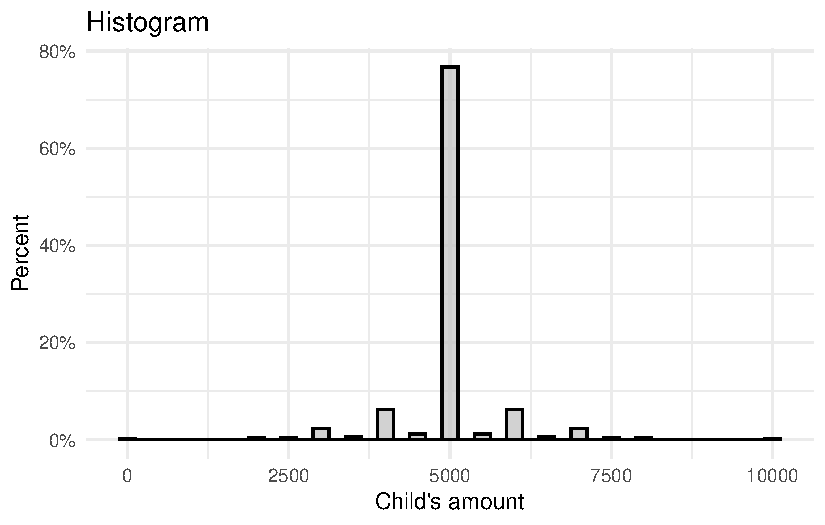
\includegraphics[keepaspectratio]{4_uebungsblatt_files/figure-pdf/unnamed-chunk-14-1.pdf}}

\section{Regression}\label{regression}

\subsection{Replikation von Tabelle 3}\label{replikation-von-tabelle-3}

\begin{Shaded}
\begin{Highlighting}[]
\CommentTok{\# Stellt sicher, dass die Referenzkategorie für jeden Faktor auf 2 gesetzt ist.}
\NormalTok{df}\SpecialCharTok{$}\NormalTok{g\_firstborn }\OtherTok{\textless{}{-}} \FunctionTok{relevel}\NormalTok{(}\FunctionTok{as.factor}\NormalTok{(df}\SpecialCharTok{$}\NormalTok{g\_firstborn), }\AttributeTok{ref =} \StringTok{"2"}\NormalTok{)}
\NormalTok{df}\SpecialCharTok{$}\NormalTok{g\_help }\OtherTok{\textless{}{-}} \FunctionTok{relevel}\NormalTok{(}\FunctionTok{as.factor}\NormalTok{(df}\SpecialCharTok{$}\NormalTok{g\_help), }\AttributeTok{ref =} \StringTok{"2"}\NormalTok{)}
\NormalTok{df}\SpecialCharTok{$}\NormalTok{g\_need }\OtherTok{\textless{}{-}} \FunctionTok{relevel}\NormalTok{(}\FunctionTok{as.factor}\NormalTok{(df}\SpecialCharTok{$}\NormalTok{g\_need), }\AttributeTok{ref =} \StringTok{"2"}\NormalTok{)}

\CommentTok{\# Run the regression model}
\NormalTok{model }\OtherTok{\textless{}{-}} \FunctionTok{lm}\NormalTok{(child\_vig }\SpecialCharTok{\textasciitilde{}}\NormalTok{ daughter }\SpecialCharTok{*}\NormalTok{ g\_firstborn }\SpecialCharTok{+}
\NormalTok{                      g\_help }\SpecialCharTok{*}\NormalTok{ daughter }\SpecialCharTok{+}
\NormalTok{                      g\_need }\SpecialCharTok{*}\NormalTok{ daughter, }
            \AttributeTok{data =}\NormalTok{ df)}

\CommentTok{\# Clustered standard errors}
\NormalTok{clustered\_se }\OtherTok{\textless{}{-}} \FunctionTok{coeftest}\NormalTok{(model, }\AttributeTok{vcov =}\NormalTok{ vcovCL, }\AttributeTok{cluster =} \SpecialCharTok{\textasciitilde{}}\NormalTok{ id\_resp)}

\CommentTok{\# Output the results}
\FunctionTok{summary}\NormalTok{(model)         }\CommentTok{\# Regression summary}
\end{Highlighting}
\end{Shaded}

\begin{verbatim}

Call:
lm(formula = child_vig ~ daughter * g_firstborn + g_help * daughter + 
    g_need * daughter, data = df)

Residuals:
    Min      1Q  Median      3Q     Max 
-4989.0  -287.8     0.0   287.8  4989.0 

Coefficients:
                      Estimate Std. Error t value Pr(>|t|)    
(Intercept)           4967.074     40.125 123.791  < 2e-16 ***
daughter                65.853     56.745   1.161   0.2459    
g_firstborn1            37.237     36.629   1.017   0.3094    
g_firstborn3             6.346     36.615   0.173   0.8624    
g_help1                320.686     36.613   8.759  < 2e-16 ***
g_help3               -207.280     36.619  -5.660 1.61e-08 ***
g_need1                205.191     36.615   5.604 2.23e-08 ***
g_need3               -313.954     36.599  -8.578  < 2e-16 ***
daughter:g_firstborn1  -43.583     51.792  -0.842   0.4001    
daughter:g_firstborn3  -43.583     51.792  -0.842   0.4001    
daughter:g_help1      -113.406     51.783  -2.190   0.0286 *  
daughter:g_help3      -113.406     51.783  -2.190   0.0286 *  
daughter:g_need1       108.763     51.770   2.101   0.0357 *  
daughter:g_need3       108.763     51.770   2.101   0.0357 *  
---
Signif. codes:  0 '***' 0.001 '**' 0.01 '*' 0.05 '.' 0.1 ' ' 1

Residual standard error: 691.3 on 4270 degrees of freedom
Multiple R-squared:  0.1624,    Adjusted R-squared:  0.1599 
F-statistic:  63.7 on 13 and 4270 DF,  p-value: < 2.2e-16
\end{verbatim}

\begin{Shaded}
\begin{Highlighting}[]
\FunctionTok{print}\NormalTok{(clustered\_se)    }\CommentTok{\# Results with clustered SE}
\end{Highlighting}
\end{Shaded}

\begin{verbatim}

t test of coefficients:

                       Estimate Std. Error  t value  Pr(>|t|)    
(Intercept)           4967.0737    37.3969 132.8206 < 2.2e-16 ***
daughter                65.8526    74.7937   0.8805   0.37866    
g_firstborn1            37.2371    43.2121   0.8617   0.38889    
g_firstborn3             6.3457    43.4854   0.1459   0.88399    
g_help1                320.6862    38.9626   8.2306 2.449e-16 ***
g_help3               -207.2799    37.9277  -5.4651 4.889e-08 ***
g_need1                205.1905    38.6142   5.3139 1.128e-07 ***
g_need3               -313.9540    39.6818  -7.9118 3.208e-15 ***
daughter:g_firstborn1  -43.5827    76.4992  -0.5697   0.56890    
daughter:g_firstborn3  -43.5827    76.4992  -0.5697   0.56890    
daughter:g_help1      -113.4063    58.6378  -1.9340   0.05318 .  
daughter:g_help3      -113.4063    58.6378  -1.9340   0.05318 .  
daughter:g_need1       108.7634    61.2365   1.7761   0.07578 .  
daughter:g_need3       108.7634    61.2365   1.7761   0.07578 .  
---
Signif. codes:  0 '***' 0.001 '**' 0.01 '*' 0.05 '.' 0.1 ' ' 1
\end{verbatim}

\begin{Shaded}
\begin{Highlighting}[]
\FunctionTok{tab\_model}\NormalTok{(model)}
\end{Highlighting}
\end{Shaded}

\begin{longtable}[]{@{}
  >{\centering\arraybackslash}p{(\linewidth - 6\tabcolsep) * \real{0.2500}}
  >{\centering\arraybackslash}p{(\linewidth - 6\tabcolsep) * \real{0.2500}}
  >{\centering\arraybackslash}p{(\linewidth - 6\tabcolsep) * \real{0.2500}}
  >{\centering\arraybackslash}p{(\linewidth - 6\tabcolsep) * \real{0.2500}}@{}}
\toprule\noalign{}
\endhead
\bottomrule\noalign{}
\endlastfoot
~ &
\multicolumn{3}{>{\centering\arraybackslash}p{(\linewidth - 6\tabcolsep) * \real{0.7500} + 4\tabcolsep}@{}}{%
\begin{minipage}[t]{\linewidth}\centering
Child\textquotesingle s amount of inter\\
vivos\strut
\end{minipage}} \\
Predictors & Estimates & CI & p \\
(Intercept) & 4967.07 & 4888.41~--~5045.74 & \textbf{\textless0.001} \\
\begin{minipage}[t]{\linewidth}\raggedright
Focal vignette person\\
daughter\strut
\end{minipage} & 65.85 & -45.40~--~177.10 & 0.246 \\
\begin{minipage}[t]{\linewidth}\raggedright
g firstborn: g firstborn\\
1\strut
\end{minipage} & 37.24 & -34.58~--~109.05 & 0.309 \\
\begin{minipage}[t]{\linewidth}\raggedright
g firstborn: g firstborn\\
3\strut
\end{minipage} & 6.35 & -65.44~--~78.13 & 0.862 \\
g help: g help 1 & 320.69 & 248.91~--~392.47 &
\textbf{\textless0.001} \\
g help: g help 3 & -207.28 & -279.07~--~-135.49 &
\textbf{\textless0.001} \\
g need: g need 1 & 205.19 & 133.41~--~276.98 &
\textbf{\textless0.001} \\
g need: g need 3 & -313.95 & -385.71~--~-242.20 &
\textbf{\textless0.001} \\
daughter:g\_firstborn1 & -43.58 & -145.12~--~57.96 & 0.400 \\
daughter:g\_firstborn3 & -43.58 & -145.12~--~57.96 & 0.400 \\
daughter:g\_help1 & -113.41 & -214.93~--~-11.89 & \textbf{0.029} \\
daughter:g\_help3 & -113.41 & -214.93~--~-11.89 & \textbf{0.029} \\
daughter:g\_need1 & 108.76 & 7.27~--~210.26 & \textbf{0.036} \\
daughter:g\_need3 & 108.76 & 7.27~--~210.26 & \textbf{0.036} \\
Observations &
\multicolumn{3}{>{\raggedright\arraybackslash}p{(\linewidth - 6\tabcolsep) * \real{0.7500} + 4\tabcolsep}@{}}{%
4284} \\
R\textsuperscript{2} / R\textsuperscript{2} adjusted &
\multicolumn{3}{>{\raggedright\arraybackslash}p{(\linewidth - 6\tabcolsep) * \real{0.7500} + 4\tabcolsep}@{}}{%
0.162 / 0.160} \\
\end{longtable}

\section{Render}\label{render}

Wandle dieses Dokument in ein PDF und ein HTML Dokument um.

\section{Weiterführende Literatur}\label{weiterfuxfchrende-literatur}

\begin{itemize}
\tightlist
\item
  \href{https://r4ds.had.co.nz/}{R for Data Science}
\end{itemize}




\end{document}
